%\documentclass[5p,times]{elsarticle}
\documentclass[11pt,review,times]{elsarticle}
%\documentclass[11pt,preprint,times]{elsarticle}

%%%%%%%%%%%%%%%%%%%%%%%%%%%%%%%%%%%%%%%%%%%%%%%%%%%%%%%%%%%%%%%%%
%	Loading packages
%%%%%%%%%%%%%%%%%%%%%%%%%%%%%%%%%%%%%%%%%%%%%%%%%%%%%%%%%%%%%%%%%
\usepackage[english]{babel}
\usepackage[utf8]{inputenc}
\usepackage[T1]{fontenc}
\usepackage{graphicx}
\usepackage{amsfonts}
\usepackage{placeins} % For /Floatbarrier
\usepackage{array,booktabs}
\usepackage{url} % For better linebreaks of URLs
\usepackage{float}

\usepackage[list-units = single,range-units = single]{siunitx}
\sisetup{separate-uncertainty}

\usepackage{caption}
\usepackage{subcaption}
\usepackage{upgreek}
\usepackage[inline]{enumitem}
\usepackage{chemformula}
%\usepackage{mathrsfs}
%\usepackage{wasysym}

\usepackage{pdfpages}


% Packages for tikz
\usepackage{tikz}
\usepackage{pgf}
\usepackage{pgfplots}
\usepackage{pgfplotstable}
	\pgfplotstableset{col sep=comma} % call once in your preamble if all your tables use commas as column separator
	\pgfplotstableset{search path={datafiles}} % Put .csv files in /datafiles or the root folder
\usetikzlibrary{3d}
\usetikzlibrary{calc}
\usetikzlibrary{decorations.pathmorphing} % Pour obtenir des lignes de coupes aléatoires
\usetikzlibrary{arrows}
\usetikzlibrary{arrows.meta,shapes,positioning,shadows,trees,decorations.pathmorphing}
\usetikzlibrary{external}
\tikzexternalize[prefix=TikzPictures/]

\biboptions{sort&compress}

\newcolumntype{M}[1]{>{\centering\arraybackslash}m{#1}} % Define a column style "M" (verticaly centered by m) and horizontaly

% Hyperref and parameters of PDF
\usepackage[hidelinks]{hyperref}
\hypersetup{
	pdftitle = {Resistance Welding of Thermoplastic Composites with a Nanocomposite Heating Element},
   pdfauthor = {David Brassard, Martine Dubé, Jason R Tavares},
	pdfkeywords={carbon nanotube, thermal conductivity, polymer, nanocomposite, heating element, Joule heating, electrical conductivity, Finite element analysis, composite, thermoplastic},
	pdfsubject={Resistance Welding of Thermoplastic Composites with a Nanocomposite Heating Element}
}

\graphicspath{{Figures/}}	% Root directory of the pictures 

%%%%%%%%%%%%%%%%%%%%%%%%%%%%%%%%%%%%%%%%%%%%%%%%%%%%%%%%%%%%%%%%%
%	Main document
%%%%%%%%%%%%%%%%%%%%%%%%%%%%%%%%%%%%%%%%%%%%%%%%%%%%%%%%%%%%%%%%%
\begin{document}
\hyphenation{COMSOL na-no-com-po-si-te na-no-com-po-si-tes}


\title{Resistance Welding of Thermoplastic Composites with a Nanocomposite Heating Element}
\journal{Composites Part B: Engineering}

\author[polymtl,crepec]{David~Brassard}
\ead{david.brassard@polymtl.com}
\author[ets,crepec]{Martine~Dubé}
\ead{martine.dube@etsmtl.ca}
\author[polymtl,crepec]{Jason~R.~Tavares\corref{cor1}}
\ead{jason.tavares@polymtl.ca}

\cortext[cor1]{Corresponding author}

\address[polymtl]{Department of Chemical Engineering, Polytechnique Montréal, P.O. Box 6079 Station Centre-Ville, Montréal, QC, H3C 3A7, Canada}
\address[ets]{Department of Mechanical Engineering, École de technologie supérieure, 1100 Notre-Dame Street West, Montréal, Québec, Canada, H3C 1K3}
\address[crepec]{Research Center for High Performance Polymer and Composite Systems (CREPEC), Polytechnique Montréal, P.O. Box 6079 Station Centre-Ville, Montréal, QC, H3C 3A7, Canada}

\begin{abstract}

This work presents the proof of concept for a PEI/MWCNT-based nanocomposite heating element for resistance welding of high performance thermoplastic composites. 
Nanocomposites with different weight fraction of MWCNTs were produced to evaluate their electrical conductivity and a composition of 10\% wt. fraction of MWCNTs achieving an electrical conductivity of \SI[multi-part-units = single]{0.79(06)}{\siemens\per\cm} was selected. 
Initial Joule heating tests with a flat nanocomposite heating element demonstrated uniform temperature at the macroscopic scale. 
At the coupon scale, single lap shear specimens with unidirectional CF/PEEK adherents were welded with the PEI/MWCNT nanocomposite heating element. 
Apparent lap shear strength up to \SI{19.6}{\mega\pascal} were obtained. 
Cohesive failure within the nanocomposite was observed and FTIR tests confirmed the absence of important thermal degradation. 

\end{abstract}

\begin{keyword}
Resistance welding;  A. Polymer–matrix composites (PMCs);  A. Thermoplastic resin;  E. Joints/joining;  
\end{keyword}

\maketitle

%%%%%%%%%%%%%%%%%%%%%%%%%%%%%%%%%%%%%%%%%%%%%%%%%%%%%%%%%%%%%%%%%
							\section{Introduction}
%%%%%%%%%%%%%%%%%%%%%%%%%%%%%%%%%%%%%%%%%%%%%%%%%%%%%%%%%%%%%%%%%

The current fierce competition in the space industry is putting a strong downward pressure on the launch cost of satellites. 
New processes and materials are needed to achieve launchers weight and cost reductions. 
Fibre reinforced polymers are commonly used to achieve weight reduction. 
Currently, thermoset polymers dominate the market for composite matrices but thermoplastic composites (TPC) are attracting the attention of the industry \cite{CompositeWorldSloan2018} because of their higher impact resistance, increased production rates, superior recyclability and higher environmental resistance \cite{cogswell1992}. 
Moreover, a distinct advantage of thermoplastics over thermosets is their ability to be joined by welding instead of adhesive bonding or mechanical fastening. 

Different welding processes have been developed for various applications and joint geometry. 
Resistance welding, induction welding and ultrasonic welding are a few of the processes used for joining TPC. 
To weld the adherents (i.e. the parts to be joined) through resistance welding (Fig. \ref{fig:welding_jig_schematic}), heat is generated by a porous heating element located at the weld interface and connected to a power source. 
An electrical current is applied to generate heat in the heating element. 
The connection between the power supply and the heating element is generally established by copper connectors that are clamped at a predetermined distance from the sides of the adherents (the so-called “clamping distance”). 
During the welding process, pressure is applied to the weld stack to achieve intimate contact between the adherents and to promote autohesion during the melting and consolidation phases. 

The first heating elements that were used for the resistance welding process were made of carbon fibre  \cite{Ageorges2000a,houghton1984bonding,Eveno1988}.
Poor weld reproducibility and problematic electrical connections between the electrodes and the carbon fibres caused scaling issues \cite{McKnight1997}. 
These shortcomings led to the use of stainless steel (SS) mesh heating elements that increased the consistency of the process \cite{Hou1999a}.

Lap shear strength (LSS) from single lap shear (SLS) tests and failure modes are commonly reported to evaluate the performance of welded joints. 
For samples welded with SS heating elements under suboptimal conditions, adhesive failure (ADH) between the mesh and the polymer or between the polymer and the adherents is obtained. 
These failure modes can be accompanied by tearing of the mesh. 
Under good welding conditions, light-fiber-tear failure (LFT), often accompanied by mesh tearing, is observed \cite{Shi2014}. 
Failure modes and LSS are dependant on the fibre nature and orientation within the adherent \cite{Shi2013a}. 
For materials with lower performances, such as glass fibre and polyetherimide (GF/PEI), rupture occurs in the adherents, but for high performance and stiffer materials, such as unidirectional carbon fibre and poly(ether ether ketone) (CF/PEEK) laminates, damage occurs in the heating element with little to no damage to the adherents \cite{Dube2015}. 
The variations in the failure modes indicate that poor adhesive bonding between the polymer and the SS mesh \cite{Dube2007,Dube2012a,Dube2009a,Shi2014,Shi2015a} can be a limiting factor under certain circumstances. 
An increase in the fraction of open area of the SS mesh, to a certain extent, improves LSS. 
Concurrently, some concerns were expressed regarding the weight penalty of SS meshes and their long-term galvanic corrosion resistance \cite{Stavrov2005a}. 
The risks of galvanic corrosion between mild steel and carbon fibres are documented \cite{Tavakkolizadeh2001,Arronche2013} but no literature, at the moment, explores the potential for galvanic corrosion between carbon fibres and stainless steel. 

Players from the space industry are looking at alternative heating elements.  
Their target is a low-density material that is not affected by corrosion. 
A conductive polymer-based nanocomposite heating element, compatible with the adherents, could serve as that alternative and provide good interfacial bonding. 
Such nanocomposites are formed by dispersing conductive nanoparticles (typically metal or carbon) into a polymer matrix. 
The electrical properties of nanocomposites depend, among other things, on the intrinsic properties of the nanoparticles, their mass fraction, surface modifications, and the mixing method employed. 
This was illustrated by Bauhofer et al., who showed that the same kinds of particles can produce nanocomposites with wildly different properties \cite{Bauhofer2009}. 
For applications such as resistance welding, we seek a conductivity sufficiently low to generate heat loads through the Joule effect but high enough to prevent current leakage through the adherents. 

For traditional resistance welding of high performance TPC parts made of CF/PEEK, PEI is commonly used to provide a resin-rich region at the weld interface. 
The miscibility of PEI in PEEK \cite{Crevecoeur1991} also improves the bonding between the adherents to attain good mechanical performances. 
By using PEI, for the matrix of the nanocomposite, we hypothesize that we could take advantage of that miscibility and obtain a nanocomposite heating element suitable for resistance welding of CF/PEEK laminates while welding at temperature lower than the melting temperature of PEEK (in a similar way to the Thermabond process \cite{Smiley1991a}). 
This novel heating element would be almost entirely miscible within the matrix of the composite. 

Herein, this article presents the development of a new heating element for resistance welding of TPC based on a conductive PEI-based polymer nanocomposite. 
The core phenomena is validated with the joule heating of a nanocomposite sample heating element. 
This new heating element is then used to join high performance TPC adherents and their mechanical performance is evaluated with single lap shear tests. 

%%%%%%%%%%%%%%%%%%%%%%%%%%%%%%%%%%%%%%%%%%%%%%%%%%%%%%%%%%%%%%%%%
							\section{Methodology}
%%%%%%%%%%%%%%%%%%%%%%%%%%%%%%%%%%%%%%%%%%%%%%%%%%%%%%%%%%%%%%%%%

%%%%%%%%%%%%%%%%%%%%%%%%%%%%%%%%%%%%%%%%%%%%%%%%%%%%%%%%%%%%%%
\subsection{Materials}
%%%%%%%%%%%%%%%%%%%%%%%%%%%%%%%%%%%%%%%%%%%%%%%%%%%%%%%%%%%%%%

\subsubsection{Polymers and Nanocomposite}

The polymer material was PEI (CAS 61128-46-9) pellets ordered from Sigma Aldrich. 
PEI pellets had a melt index of \SI{18}{\gram} per \SI{10}{\minute} at \SI{337}{\celsius} with a mass of \SI{6.6}{\kilogram}. 
GPC/SEC measurements of the molecular weight for this PEI gave a $M_n$ of \textbf{XXXXXXX} and a $M_w$ of \textbf{XXXXXXX}. 

The conductive nanoparticles consisted of dry powdered MWCNTs, produced by combustion chemical vapour deposition (CCVD), purchased from Raymor Industries. 
They had outer diameters in the range of \SIrange{10}{20}{\nano\metre}, lengths from \SIrange{1}{12}{\micro\metre} and purity of at least 99\%.

Initial batches of nanocomposites with 5\%, 10\% and 15\% wt. of MWCNTs were produced with a DSM Xplore 5~cc twin-screw micro compounder. 
Polymer pellets were introduced along with the MWCNTs and internally mixed by the recirculation circuit.
The resulting extruded wire was cut into pellets that were mixed and fed a second time to produce a uniform mix for each batch. 
The pellets were pressed to produce \SI{1.6}{\mm} thick flat samples to measure their electrical conductivity.  

The electrical conductivity of the PEI nanocomposites, at 5\%, 10\% and 15\% wt. of MWCNTs, was measured with the four-point probe technique. 
A probe manufactured by Jandel engineering was mounted on a resistivity test rig from A\&M Fell Ltd. and connected to an acquisition system composed of a Keithley 220 programmable current source and a Hewlett Packard 34401A multimeter. 
The tungsten carbide probes had a diameter of \SI{0.4}{\mm}, a radius of \SI{100}{\um} and a spacing of \SI{1}{\mm}. 

The final batch of nanocomposite with 10\% wt. of MWCNTs was produced in a twin-screw extruder and processed at \SI{340}{\celsius}. 
Polymer pellets were introduced along with the MWCNTs. 
The extruded wire was cut into small pellets, mixed thoroughly and fed back into the extruder two other times to obtain a uniform composition. 
The final wire was cut into pellets prior further processing. 
Flat PEI nanocomposite heating elements, with a 10\% mass fraction of MWCNTs, were produced by hot pressing pellets into \SI{0.5}{\milli\metre} thick films and cutting them into rectangles of \SI{12.7 x 55}{\milli\metre}. 

\subsubsection{Composite}

The TPC adherents were produced by hot pressing CF/PEEK pre-impregnated plies to form unidirectional (UD) composite laminates and cutting them to dimensions (\SI{25.4 x 101.6}{\milli\metre} ), with an abrasive saw, according to ASTM D5868 - 01(2014). 
In agreement with the supplier’s recommendations, the stacks of plies were heated to \SI{390}{\celsius} under a pressure of \SI{0.25}{\MPa}. 
The pressure was then increased to \SI{2}{\MPa} for \SI{30}{\minute} to consolidate the laminate before cooling it back to room temperature in about \SI{60}{\minute}. 
The pressure was maintained during the cooling phase. 

%%%%%%%%%%%%%%%%%%%%%%%%%%%%%%%%%%%%%%%%%%%%%%%%%%%%%%%%%%%%%%
\subsection{Joule Heating of a Nanocomposite Heating Element}
%%%%%%%%%%%%%%%%%%%%%%%%%%%%%%%%%%%%%%%%%%%%%%%%%%%%%%%%%%%%%%

Prior to the welding tests, a simple validation of the heating elements was devised. 
A \SI{0.5}{\milli\metre} thick PEI heating element, was installed in the welding system with a programmable DC power source. 
The electrodes were then lowered and pressed against the nanocomposite with a gap of \SI{25}{\mm} between them. 
The strength of the electrical field was obtained by dividing the voltage from the source by the distance between the electrodes. 
A FLIR T420 infrared camera was used to record the surface temperature distribution. 

%%%%%%%%%%%%%%%%%%%%%%%%%%%%%%%%%%%%%%%%%%%%%%%%%%%%%%%%%%%%%%
\subsection{Welding Experiments}
%%%%%%%%%%%%%%%%%%%%%%%%%%%%%%%%%%%%%%%%%%%%%%%%%%%%%%%%%%%%%%

A computer-controlled resistance welding jig was built to weld single lap shear test samples with an overlap of \SI{12.7}{\milli\metre} and a width of \SI{25.4}{\milli\metre} (Fig. \ref{fig:welding_jig}). 
Two square-ended copper electrodes (\SI{12.7}{\milli\metre} $\times$ \SI{12.7}{\milli\metre}) were used to connect the power source to the nanocomposite heating element. 
Three pneumatic actuators applied constant pressure over the two electrodes and the welded zone, while the nanocomposite was kept between two composite adherents surrounded by \SI{12.7}{\milli\metre} thick alumina silicate ceramic insulating blocks. 
The section of the nanocomposite heating element outside of the welded zone, on each side (Fig. \ref{fig:location_thermocouple}), where the electrodes were connected, rested flat on the insulating blocks. 
These tabs are where the electrodes were connected; the clamping distances (Fig. \ref{fig:welding_jig_schematic}), on each sides of the adherent, between the faces of the electrodes and the sides of the adherent were adjusted for each test. 
Electrical power was supplied by a \SI{10}{\kW} programmable DC power source series XR from Magna-Power capable of providing up to \SI{160}{\volt} and \SI{60}{\ampere}. 
The power source can be driven as a constant voltage source, constant current source or with custom power profiles. 
A modulation scheme was configured to allow the source to operate with a constant power output. 
In this mode of operation, the source adjusts its output current based on the voltage applied and keeps a constant power output, disregarding variations in the resistance of the heating element. 

For the welding experiments, electrical parameters were set so as to closely mimic conditions that are observed during traditional resistance welding of TPC. 
The initial voltage setting for constant voltage operation was calculated based on a specific power of \SI{350}{\kW\per\square\metre} and the electrical resistance of the heating element. 

Prior to welding, the surfaces of the adherents and the nanocomposite were thoroughly cleaned with acetone to remove any traces of residue or release agent. 
Once assembled, a contact pressure of 2.4 MPa was applied by the electrodes, to minimize contact resistance. 
Over the weld area, a third actuator applied a constant pressure of \SI{1}{\MPa} during the whole welding process. 
It was previously demonstrated, for traditional resistance welding, that pressures close to \SI{1}{\MPa} are able to produce welds with good mechanical properties by promoting intimate contact, necessary for polymer chain transfer at the interfaces, while preventing void formation due to excessive polymer flow out of the weld \cite{Ageorges2000a, Dube2007, Shi2014}. 
Type K thermocouples, located on the ceramic above the welded zone, monitored the temperature during the welding process (Fig. \ref{fig:location_thermocouple}). 
The thermocouples could not be installed directly on the nanocomposite heating element, as their presence altered the heat transfer mechanisms within the weld and Kapton\textregistered \ tape was not sufficient to isolate them from electrical interferences. 
The first thermocouple was located slightly off centre at \SI{14}{\milli\metre} from the side of the adherent at the centreline of the overlap. 
The second thermocouple was also located on the centreline, but \SI{2.5}{\milli\metre} away from the side of the adherent. 
These two location served as proxy to approximate the temperature within the weld but a higher temperature is expected to occur within the joint. 

Aside from the operating mode for the power source, the electrode distance from the side of the laminate and the duration of the welding process were the main factors taken into account during the welding tests. 
The LSS of each weld was evaluated with a SLS test as per ASTM D5868 – 01(2014) with an MTS Alliance RF/200 testing machine. 
Subsequently, fractography analysis was carried out with ImageJ. 
In this analysis, dividing the area of the welded zone by the total area gave the percentage of welded area. 
Both sides of the fracture specimens were evaluated to get an average measure for each sample. 
The failure modes obtained were classified and reported as per ASTM D5573 – 99(2012). 

\FloatBarrier
%%%%%%%%%%%%%%%%%%%%%%%%%%%%%%%%%%%%%%%%%%%%%%%%%%%%%%%%%%%%%%
\subsection{FTIR Analysis}
%%%%%%%%%%%%%%%%%%%%%%%%%%%%%%%%%%%%%%%%%%%%%%%%%%%%%%%%%%%%%%

FTIR spectra were collected to validate the absence of thermal degradation induced by the welding process. 
A Nicolet iS5 FTIR Spectrometer equipped with an iD5 attenuated total reflectance (ATR) module was used to collect spectra from the virgin PEI pellets and PEI nanocomposite films before welding, and PEI nanocomposite on the fracture surface after SLS tests. 
Spectra for CF/PEEK adherents were also collected to serve as reference.  

\FloatBarrier
%%%%%%%%%%%%%%%%%%%%%%%%%%%%%%%%%%%%%%%%%%%%%%%%%%%%%%%%%%%%%%%%%
							\section{Results and Discussion}
%%%%%%%%%%%%%%%%%%%%%%%%%%%%%%%%%%%%%%%%%%%%%%%%%%%%%%%%%%%%%%%%% 

%%%%%%%%%%%%%%%%%%%%%%%%%%%%%%%%%%%%%%%%%%%%%%%%%%%%%%%%%%%%%%
\subsection{Electrical Conductivity of the Nanocomposites}
%%%%%%%%%%%%%%%%%%%%%%%%%%%%%%%%%%%%%%%%%%%%%%%%%%%%%%%%%%%%%%

The electrical conductivity of PEI nanocomposites with 5\%, 10\% and 15\% wt. MWCNTs was measured at respectively of \SIlist[multi-part-units = single]{0.27(08);0.79(06);0.92(30)}{\siemens\per\cm}. 
It was decided that the marginal gain in conductivity between 10\% and 15\% wt. MWCNTs was not worth the increased cost and production problems associated with high particle loading (such as increased viscosity and brittleness). 
Thus, PEI nanocomposite films with 10\% wt. MWCNTs were retained for the welding tests. 

%%%%%%%%%%%%%%%%%%%%%%%%%%%%%%%%%%%%%%%%%%%%%%%%%%%%%%%%%%%%%%
\subsection{Joule Heating of a Nanocomposite Heating Element}
%%%%%%%%%%%%%%%%%%%%%%%%%%%%%%%%%%%%%%%%%%%%%%%%%%%%%%%%%%%%%%

Taking into account the edge effects from the electrodes, uniform heating of the nanocomposite was observed during this experiment (Fig. \ref{fig:results_lab}). 
It was also possible to control the surface temperature of the heating element with a variation of the electrical field (Tab. \ref{tab:results_lab}). 

\FloatBarrier

%%%%%%%%%%%%%%%%%%%%%%%%%%%%%%%%%%%%%%%%%%%%%%%%%%%%%%%%%%%%%%
\subsection{Welding Experiments}
%%%%%%%%%%%%%%%%%%%%%%%%%%%%%%%%%%%%%%%%%%%%%%%%%%%%%%%%%%%%%%

Small geometric variations of the nanocomposite heating elements (thickness and width) introduced variations of the electrical resistance. 
Due to that, operation under constant voltage conditions achieved poor reproducibility between initial welding tests and was not investigated further. 
Operation under constant power yielded significant improvements in the consistency of welding results, avoiding the effect introduced by the resistance variation of the heating element. 

\subsubsection{Constant power welding}
\FloatBarrier

Tests were carried out at a specific power of \SI{350}{\kW\per\square\metre} with a constant pressure of \SI{1}{\MPa} on the weld. 
Clamping distances of \SIlist{0;1;1.5}{\mm} and welding times of \SIlist{60;70;90;120}{\s} were investigated. 
Three samples were produced for each welding condition. 
The LSS along with the average fraction of welded areas are reported in Table \ref{tab:SLS_and_fractography_results}. 

Cohesive failure within the nanocomposite was the primary mode of rupture observed for samples welded under constant power with UD composite adherents.
Some adhesive failure on the edges of the heating element was also observed. 
Samples welded for \SI{60}{\s} with a clamping distance of \SI{1.5}{\mm} presented a higher fraction of adhesive failure. 
The zone where cohesive failure is observed had an hourglass shape with a thinner width at the centre of the weld (Fig. \ref{fig:fracture_surface_70s}). 
For welding times of \SI{90}{\s} and longer, the hourglass shape is absent from the results and only cohesive failure of the nanocomposite is present (Fig. \ref{fig:fracture_surface_90s}). 

Temperature monitoring during the welding process of a sample with a clamping distance of \SI{1.5}{\mm} showed temperature variations between the centre and the side of the weld (Fig. \ref{fig:temp_350kW_120_10_150_3UD}).
For this specimen, the edge effect resulted in a \SI{10}{\celsius} higher temperature on the top surface at the side of the adherent. 
This difference was caused by a clamping distance that was too large. 
Models will be required to evaluate if the gradients in the weld are larger or smaller than the gradient from the thermocouples. 
Nonetheless, the temperature gradient between the center and the sides was not sufficient to lead to observable thermal degradation, in the fractography results, either on the sides (from a clamping distances too high) or at the centre of the weld (from a clamping distances too small). 
It was previously demonstrated that the clamping distance has a major impact on the heat transport phenomena at the edge of the weld.
The maximum temperature recorded, by the thermocouple, during that test (\SI{207}{\celsius}), is lower than the glass transition temperature ($T_g$ of \SI{217}{\celsius} for PEI) due to the location of the thermocouple on the surface of the adherents. 
Visual inspection of the fractography after SLS testing showed that, for that specimen, incomplete melting of the nanocomposite occurred in the interface close to an edge of the adherents. 

Although the LSS obtained with the nanocomposite heating element are not on the same level as the best results reported in the literature for traditional resistance welding (up to \SI{50}{\MPa} for UD CF/PEEK adherents \cite{Dube2015} and \SI{41}{\MPa} with the Thermabond process \cite{Smiley1991a}) successful weld were obtained with the first iteration of this process and key optimization parameters were identified for future work. 
The main parameters that could explain the lower performance of the joints are \begin{enumerate*}[label=(\arabic*)]
	\item the reduced toughness of the nanocomposite due to the addition of a high fraction of MWCNTs,
	\item the lack of complete melting in the welded zone due to improper clamping distance and other edge effects,
	\item the hourglass shape of the welded zone leading to stress concentration at the edge and
	\item the thicker joints obtained when applying a pressure of only \SI{1}{\MPa}. 
\end{enumerate*}
A reduction of 40\% of the stress at rupture during tensile tests on dogbones made from the nanocomposite showed that the addition of 10\% wt. fraction of MWCNTs has a major impact on the mechanical properties of the polymer. 
Plasticizers could be used to reduce this factor but the composition of the nanocomposite will need to be balanced as to still provide a sufficient electrical conductivity. 
Improving the control of the welding process (clamping distance, time and power density) will reduce the temperature gradients within the welded zone and provide a better wetting over the whole surface of the joint. 
Thicker joints have lower LSS then thinner joints. 
The addition of 10\% wt. fraction of MWCNTs, increased the viscosity of the PEI limiting polymer flow out of the weld. 
Thicker joints (about \SI{0.3}{\mm} vs \SI{0.15}{\mm} for traditional resistance welding) were caused by the limited pressure applied on the weld. 
A higher pressure during welding allow the production of thinner and better performing joints at the risk of creating voids if too much polymer leaves the weld. 

\subsection{FTIR results}

When comparing the FTIR spectra of PEI nanocomposite before and after the welding process, no signs of degradation could be noted (see supplementary information). 
The characteristic peeks for \ch{CH3}, \ch{CH} and \ch{C=O} in PEI were left unchanged by the welding process. 

\FloatBarrier

%%%%%%%%%%%%%%%%%%%%%%%%%%%%%%%%%%%%%%%%%%%%%%%%%%%%%%%%%%%%%%%%%
							\section{Conclusion}
%%%%%%%%%%%%%%%%%%%%%%%%%%%%%%%%%%%%%%%%%%%%%%%%%%%%%%%%%%%%%%%%%

Through this work, we have demonstrated that a PEI/MWCNT-based nanocomposite heating element could be used for resistance welding of TPCs. 
An experimental validation using a PEI/MWCNT flat heating element subjected to a DC electric field showed uniform heating. 
Resistance welding using the PEI/MWCNT heating element in a custom-built welding jig joined CF/PEEK UD panels with LSS up to \SI{19.6}{\MPa}. 
Good bonding to the adherents is supported by the cohesive failure mode observed, and no important thermal degradation is measured by FTIR tests. 
Future work will need focus on improving the temperature uniformity in the weld, studying the effect of a higher pressure over the weld and improving the toughness of the nanocomposite with the goal of increasing the mechanical resistance of the final weld.

%%%%%%%%%%%%%%%%%%%%%%%%%%%%%%%%%%%%%%%%%%%%%%%%%%%%%%%%%%%%%%%%%
							\section{Acknowledgements}
%%%%%%%%%%%%%%%%%%%%%%%%%%%%%%%%%%%%%%%%%%%%%%%%%%%%%%%%%%%%%%%%%

This work was supported by ArianeGroup and CREPEC. 
The authors also thank Prof. G.S. Patience for the use of the thermal imaging camera and Prof. D. Therriault for access to the microcompounder. 

%%%%%%%%%%%%%%%%%%%%%%%%%%%%%%%%%%%%%%%%%%%%%%%%%%%%%%%%%%%%%%%%%
							\section*{References}
%%%%%%%%%%%%%%%%%%%%%%%%%%%%%%%%%%%%%%%%%%%%%%%%%%%%%%%%%%%%%%%%%

\bibliographystyle{model4-names}
\bibliography{Article_soudage_nano_1}
%\pagebreak

%\section{Figures}
%\FloatBarrier

\pagebreak
%%%%%%%%%%%%%%%%%%%%%%%%%%%%%%%%%%%%%%%%%%%%%%%%%%%%%%%%%%%%%%%%%
							\section*{Figures}
%%%%%%%%%%%%%%%%%%%%%%%%%%%%%%%%%%%%%%%%%%%%%%%%%%%%%%%%%%%%%%%%%
\FloatBarrier


\begin{figure}[htb]
	\centering
	\captionsetup{width=125mm}
	\begin{subfigure}{65mm}
		\centering
		\captionsetup{width=65mm}
		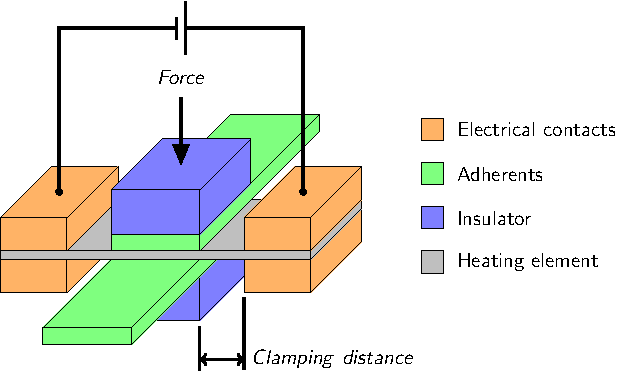
\includegraphics[width=65mm]{beamer_IC3_DBrassard-figure1.pdf}
		\caption{Resistance welding main components \cite{Brassard2018_figshare_article1}}
		\label{fig:welding_jig_schematic}
	\end{subfigure}
	\begin{subfigure}{55mm}
		\centering
		\captionsetup{width=55mm}
		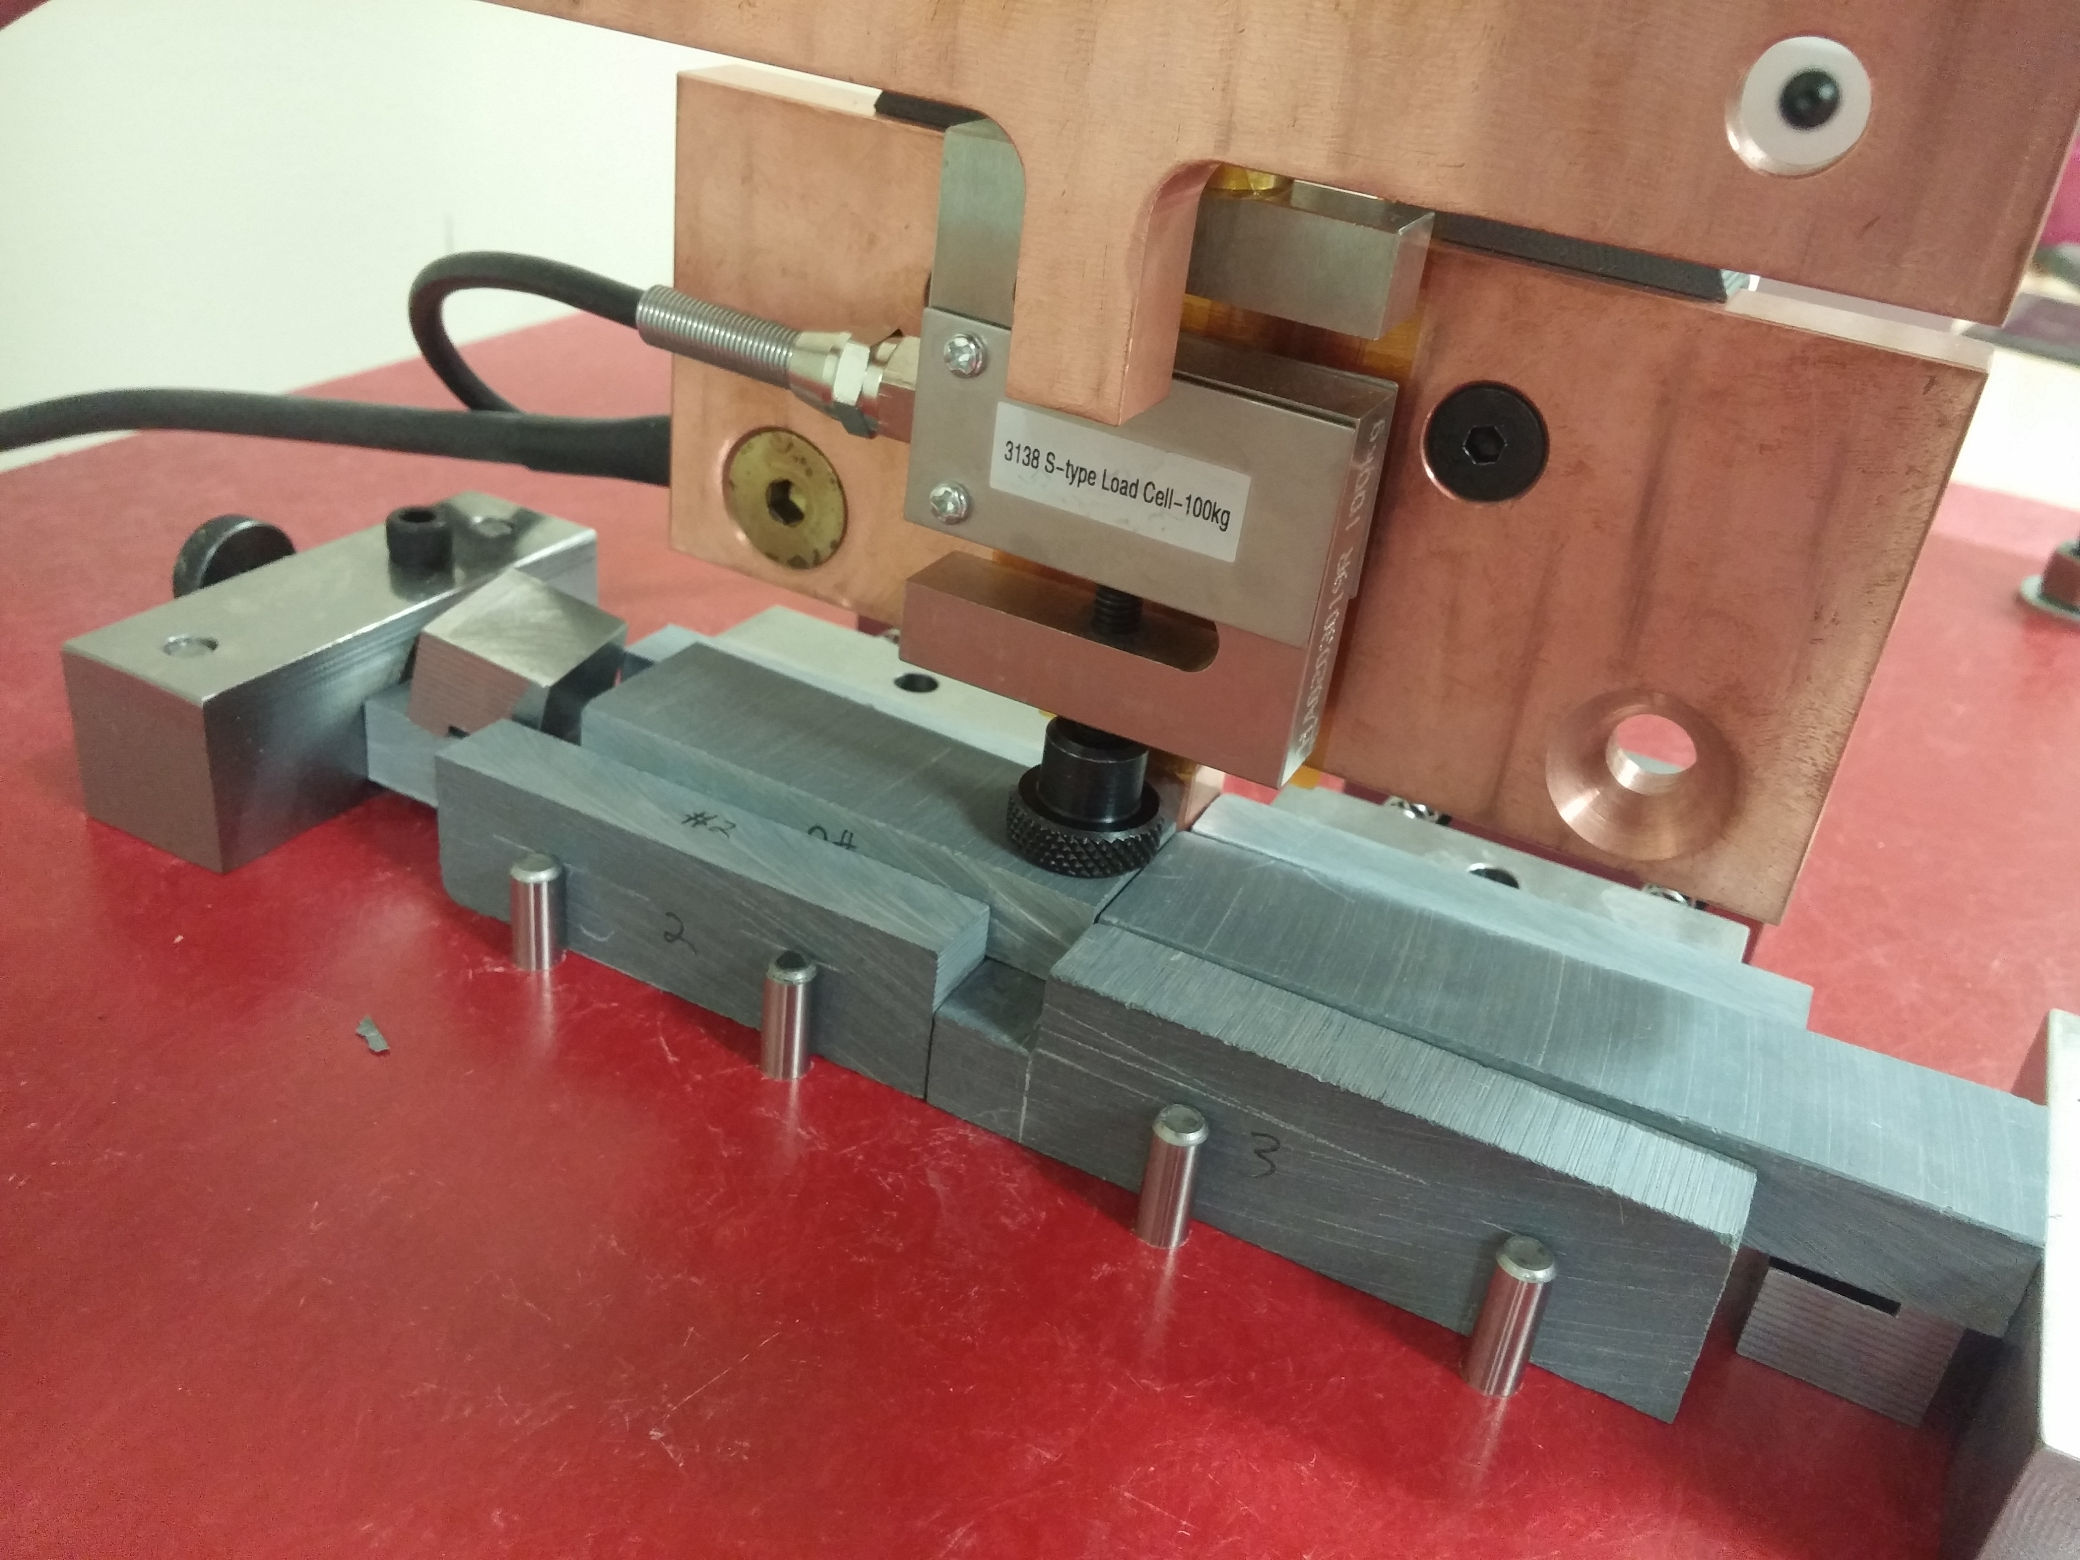
\includegraphics[width=55mm]{20161026_152818_resize.jpg}
		\caption{Ceramic insulators, copper electrodes and load cell}
		\label{fig:welding_jig_electrodes}
	\end{subfigure}%	
	\caption{Resistance welding jig \cite{Brassard2018_figshare_article1}}
	\label{fig:welding_jig}
\end{figure}

\begin{figure}
		\center
		\captionsetup{width=60mm}
		%\resizebox{60mm}{!}{
		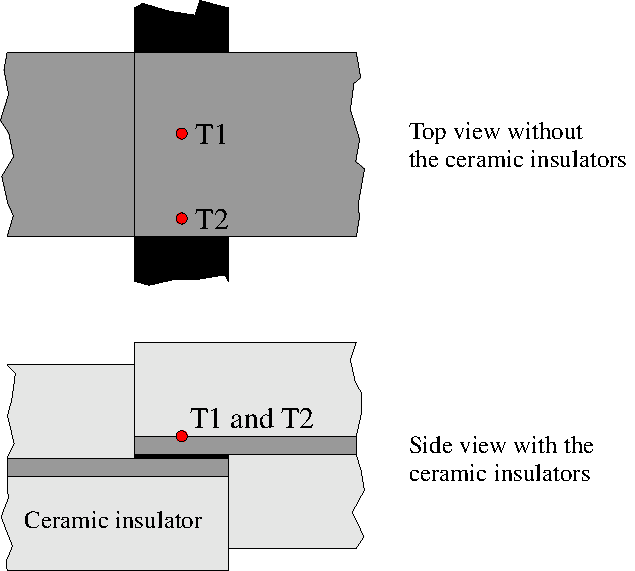
\includegraphics[width=60mm]{thermocouple_welding}
		%\tikzsetnextfilename{thermocouple_welding}
		%\usetikzlibrary{arrows.meta,shapes,positioning,shadows,trees,decorations.pathmorphing}

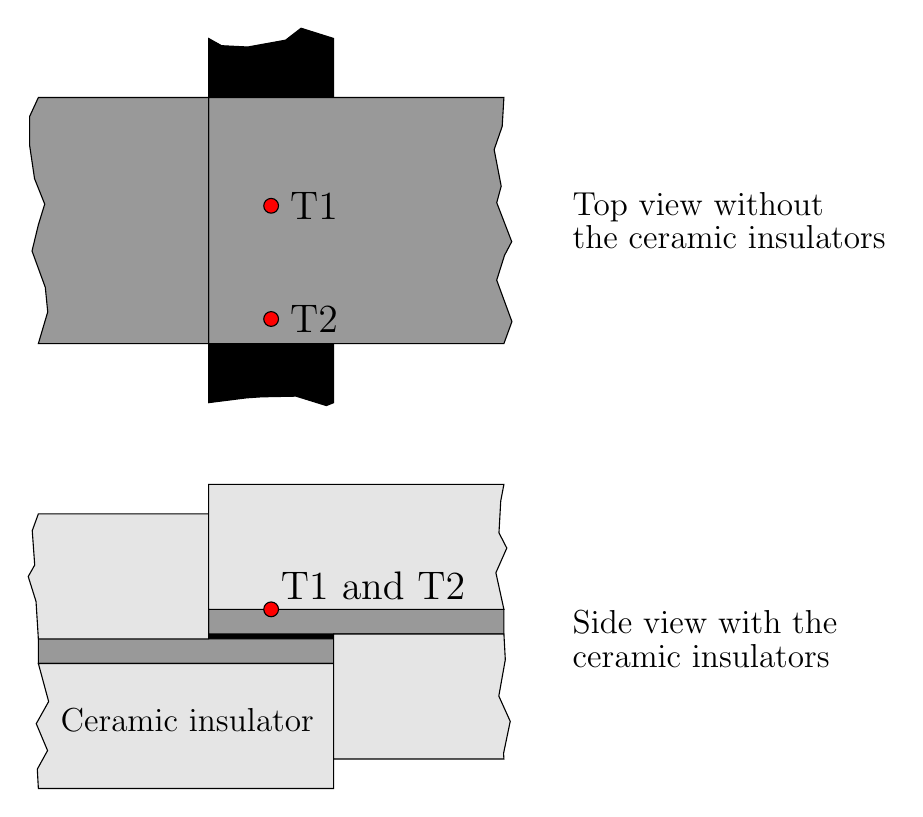
\begin{tikzpicture}[scale=0.125]

%Couleurs
\def \colceramique{black!10}
\def \colcomposite{black!40}

%Définition des dimensions du joint soudé
\def \overlap{12.7}
\def \epceramique{12.7}
\def \epcomposite{2.5}
\def \epnanocomposite{0.5}
\def \longueur{30}
\def \gapfigure{30}
\def \largeursoudure{25}
\def \depassementsoudure{6}
\def \diacercle{0.75}

%%%Vue du dessus %%%
\draw (\longueur+\depassementsoudure,\gapfigure+0.5*\largeursoudure) node [right, align=left]{\large Top view without \\ \large the ceramic insulators};

%Élément chauffant
\draw[black,decoration={random steps, amplitude=4, segment length=10},fill=black] (0,\gapfigure-\depassementsoudure) decorate{-- ++(\overlap,0)} -- ++(0,2*\depassementsoudure+\largeursoudure) decorate{-- ++(-\overlap,0)} -- cycle;

%Adhérent
\draw[black,decoration={random steps, amplitude=4, segment length=10},fill=\colcomposite] 
(0,\gapfigure) -- ++(\longueur,0) decorate{-- ++(0,\largeursoudure)} -- ++(-\longueur,0) -- cycle;
\draw[black,decoration={random steps, amplitude=4, segment length=10},fill=\colcomposite] 
(0,\gapfigure) -- ++(-\longueur+\overlap,0) decorate{-- ++(0,\largeursoudure)} -- ++(\longueur-\overlap,0) -- cycle;

%Position du thermocouple
\draw[fill=red] (0.5*\overlap,\gapfigure+14) circle (0.75) node [right]{\ \Large T1};
\draw[fill=red] (0.5*\overlap,\gapfigure+2.5) circle (0.75) node [right]{\ \Large T2};


%%% Vue du côté %%%
\draw (\longueur+\depassementsoudure,0) node [right, align=left]{\large Side view with the \\ \large ceramic insulators};

%Éléments chauffants
\draw[black,thick,fill=black] (0,0) -- ++(\overlap,0) -- ++(0,\epnanocomposite) -- ++(-\overlap,0) -- cycle;

%Adhérents
\draw[black,decoration={random steps, amplitude=4, segment length=6},fill=\colcomposite] 
(\overlap,0) -- ++(-\longueur,0) decorate{-- ++(0,-\epcomposite)} -- ++(\longueur,0) -- cycle;
\draw[black,decoration={random steps, amplitude=4, segment length=6},fill=\colcomposite] 
(0,\epnanocomposite) -- ++(\longueur,0) decorate{-- ++(0,\epcomposite)} -- ++(-\longueur,0) -- cycle;

%Céramiques
\draw[black,decoration={random steps, amplitude=4, segment length=10},fill=\colceramique] 
(\overlap,-\epcomposite) -- ++(-\longueur,0) decorate{-- ++(0,-\epceramique)} -- ++(\longueur,0) -- cycle;
\draw[black,decoration={random steps, amplitude=4, segment length=10},fill=\colceramique] 
(0,0) -- ++(-\longueur+\overlap,0) decorate{-- ++(0,\epceramique)} -- ++(\longueur-\overlap,0) -- cycle;
\draw[black,decoration={random steps, amplitude=4, segment length=10},fill=\colceramique] 
(\overlap,\epnanocomposite) -- ++(\longueur-\overlap,0) decorate{-- ++(0,-\epceramique)} -- ++(-\longueur+\overlap,0) -- cycle;
\draw[black,decoration={random steps, amplitude=4, segment length=10},fill=\colceramique] 
(0,\epnanocomposite+\epcomposite) -- ++(\longueur,0) decorate{-- ++(0,\epceramique)} -- ++(-\longueur,0) -- cycle;

%Identification des céramiques
\draw (-\longueur+1.1*\overlap,-0.65*\epceramique) node [right, align=left]{ \large Ceramic insulator};

%Position du thermocouple
\draw[fill=red] (0.5*\overlap,\epnanocomposite+\epcomposite) circle (0.75) node [above right]{\Large T1 and T2};


\end{tikzpicture}

		%}
		\caption{Location of the thermocouples during the welding process \cite{Brassard2018_figshare_article1}}
		\label{fig:location_thermocouple}
\end{figure} 

\begin{figure}[htb]
	\center
	\captionsetup{width=125mm}
	
	\begin{subfigure}{55mm}
		\center
		\captionsetup{width=50mm}
		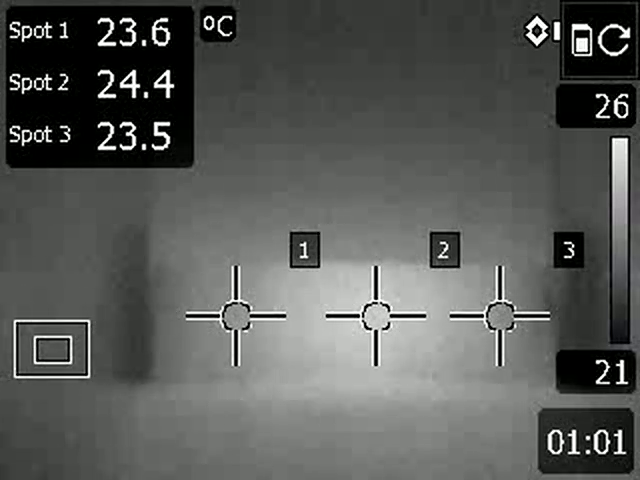
\includegraphics[width=50mm]{t_00.png}
		\caption{time = \SI{0}{\s}}
	\end{subfigure}
	\begin{subfigure}{55mm}
		\center
		\captionsetup{width=50mm}
		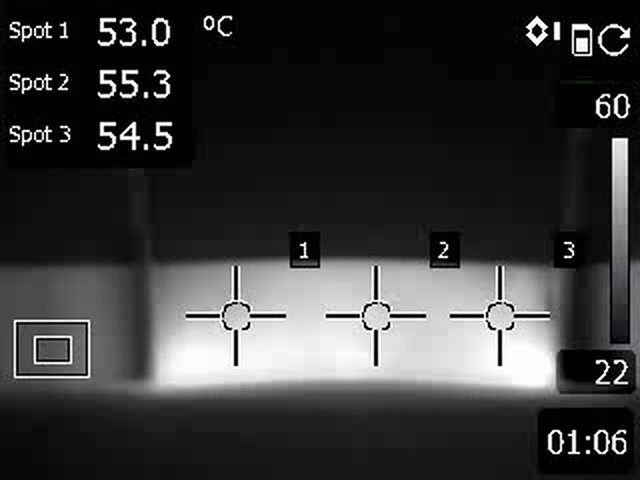
\includegraphics[width=50mm]{t_05.png}
		\caption{time = \SI{5}{\s}}
	\end{subfigure}
	\begin{subfigure}{55mm}
		\center
		\captionsetup{width=50mm}
		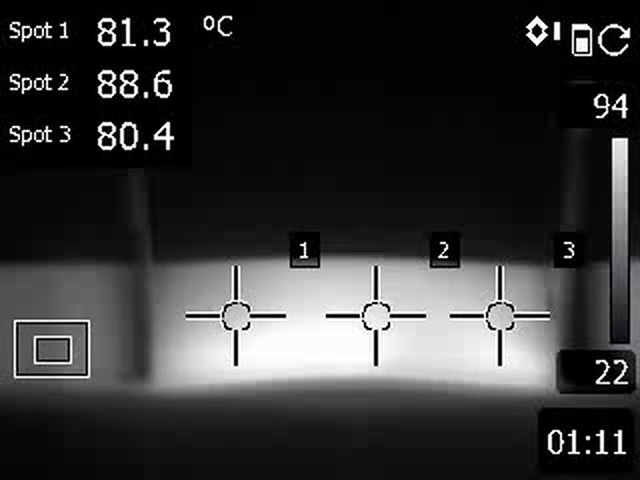
\includegraphics[width=50mm]{t_10.png}
		\caption{time = \SI{10}{\s}}
	\end{subfigure}
	\begin{subfigure}{55mm}
		\center
		\captionsetup{width=50mm}
		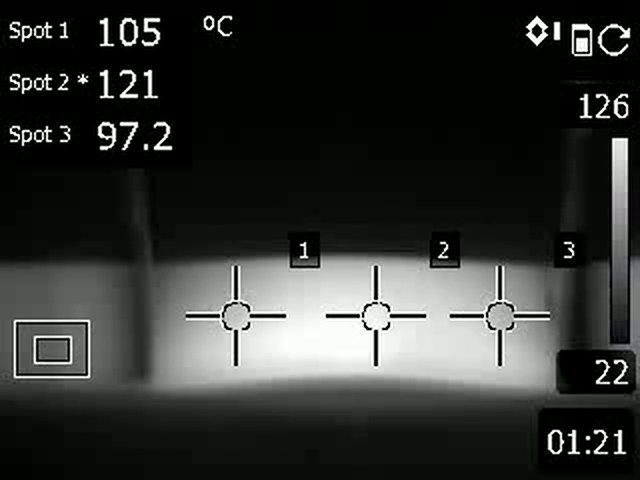
\includegraphics[width=50mm]{t_20.png}
		\caption{time = \SI{20}{\s}}
	\end{subfigure}
	\begin{subfigure}{55mm}
		\center
		\captionsetup{width=50mm}
		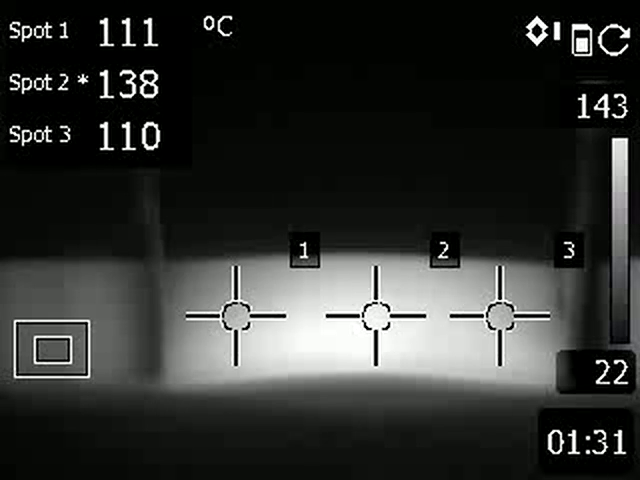
\includegraphics[width=50mm]{t_30.png}
		\caption{time = \SI{30}{\s}}
	\end{subfigure}
	\begin{subfigure}{55mm}
		\center
		\captionsetup{width=50mm}
		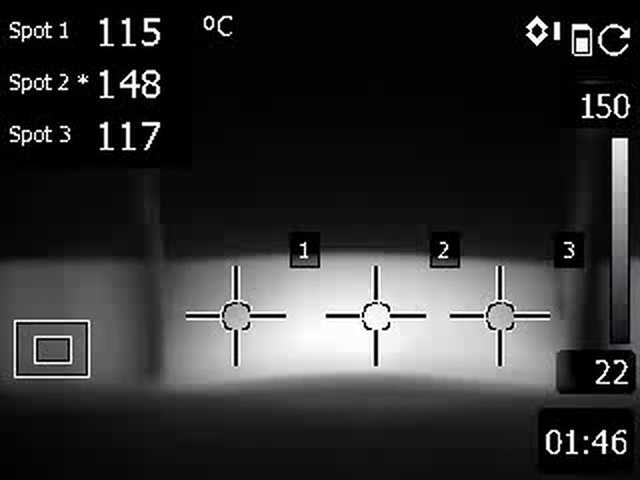
\includegraphics[width=50mm]{t_45.png}
		\caption{time = \SI{45}{\s}}
	\end{subfigure}
	\caption{Thermography of a heating element during the experimental validation under a DC electrical field of \SI{800}{\volt\per\metre} \cite{Brassard2018_figshare_article1}}
	\label{fig:results_lab}
\end{figure}

\begin{figure}[htb]
	\center
	\captionsetup{width=125mm}
	\begin{subfigure}{125mm}
		\center
		\captionsetup{width=125mm}
		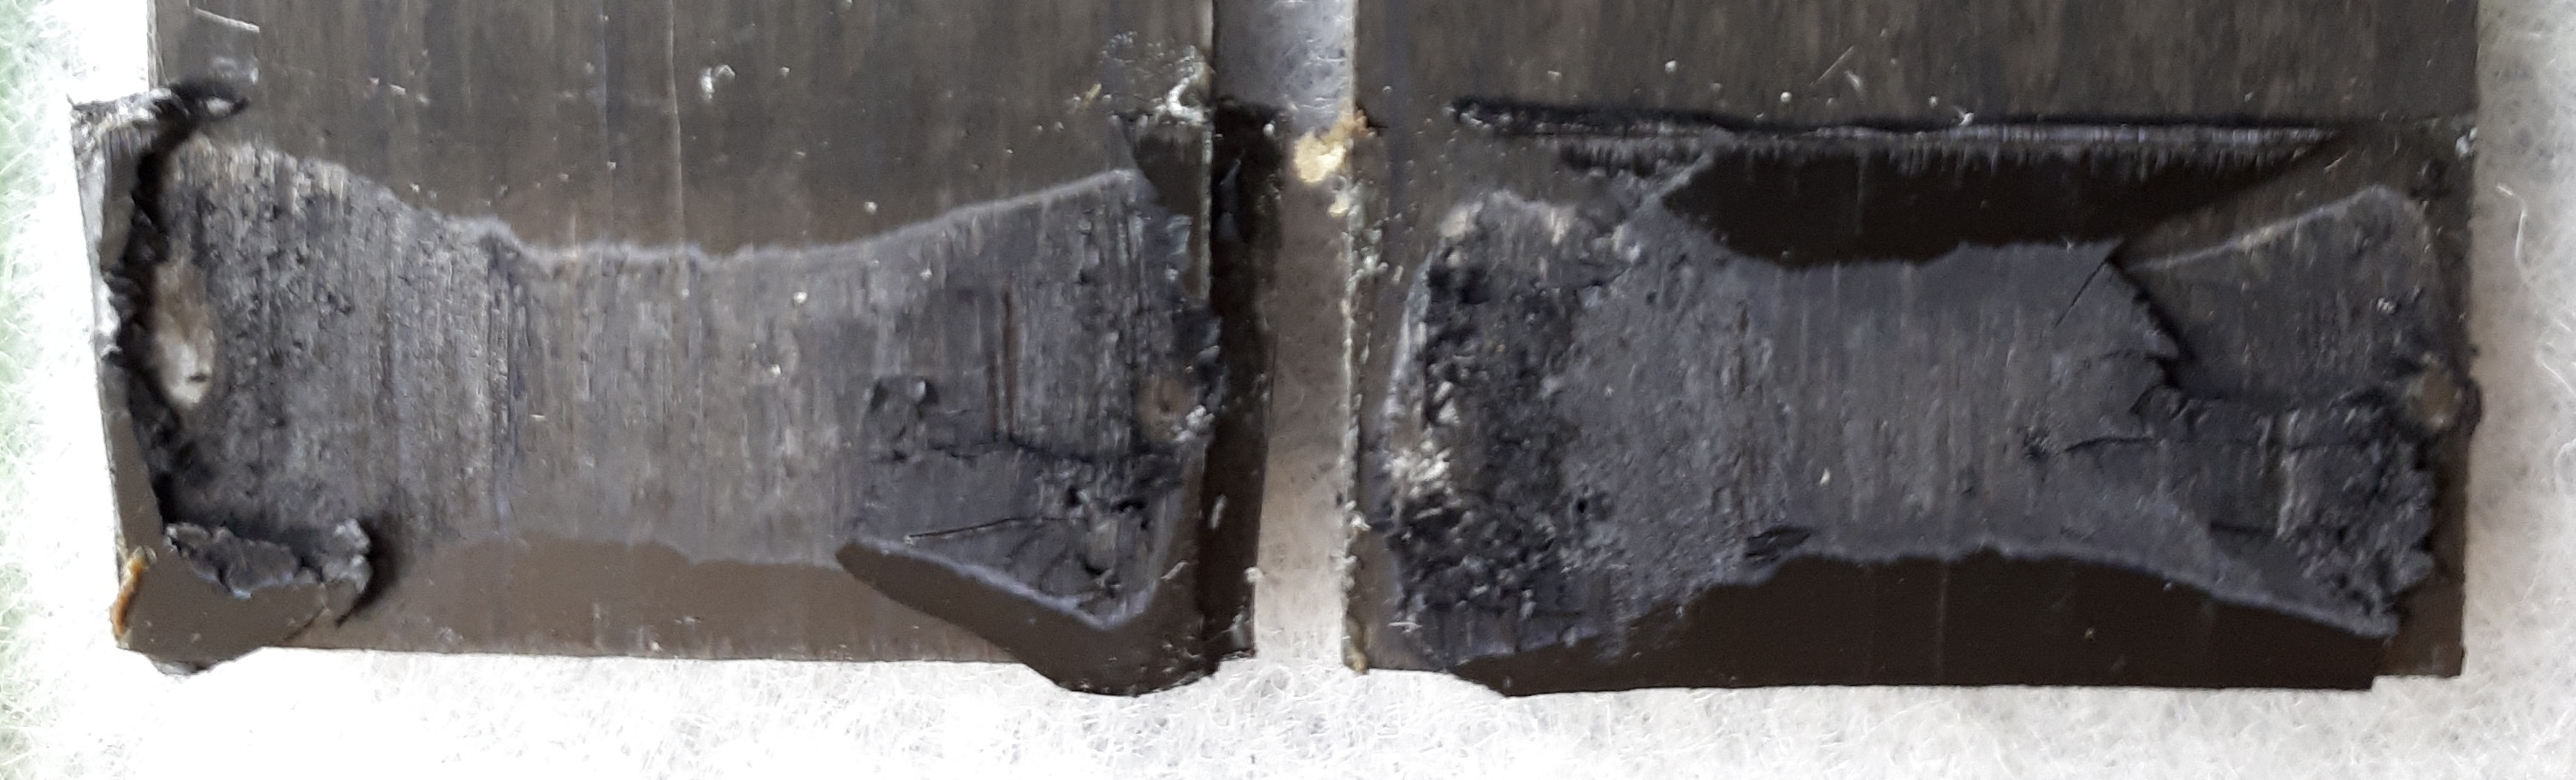
\includegraphics[width=125mm]{350kW-70-10-150-1UD_crop.jpg}
		\caption{Cohesive failure with an hourglass shape in the middle and adhesive failure on the sides in a sample welded for \SI{70}{\s}}
		\label{fig:fracture_surface_70s}
	\end{subfigure}
	\begin{subfigure}{125mm}
		\center
		\captionsetup{width=125mm}
		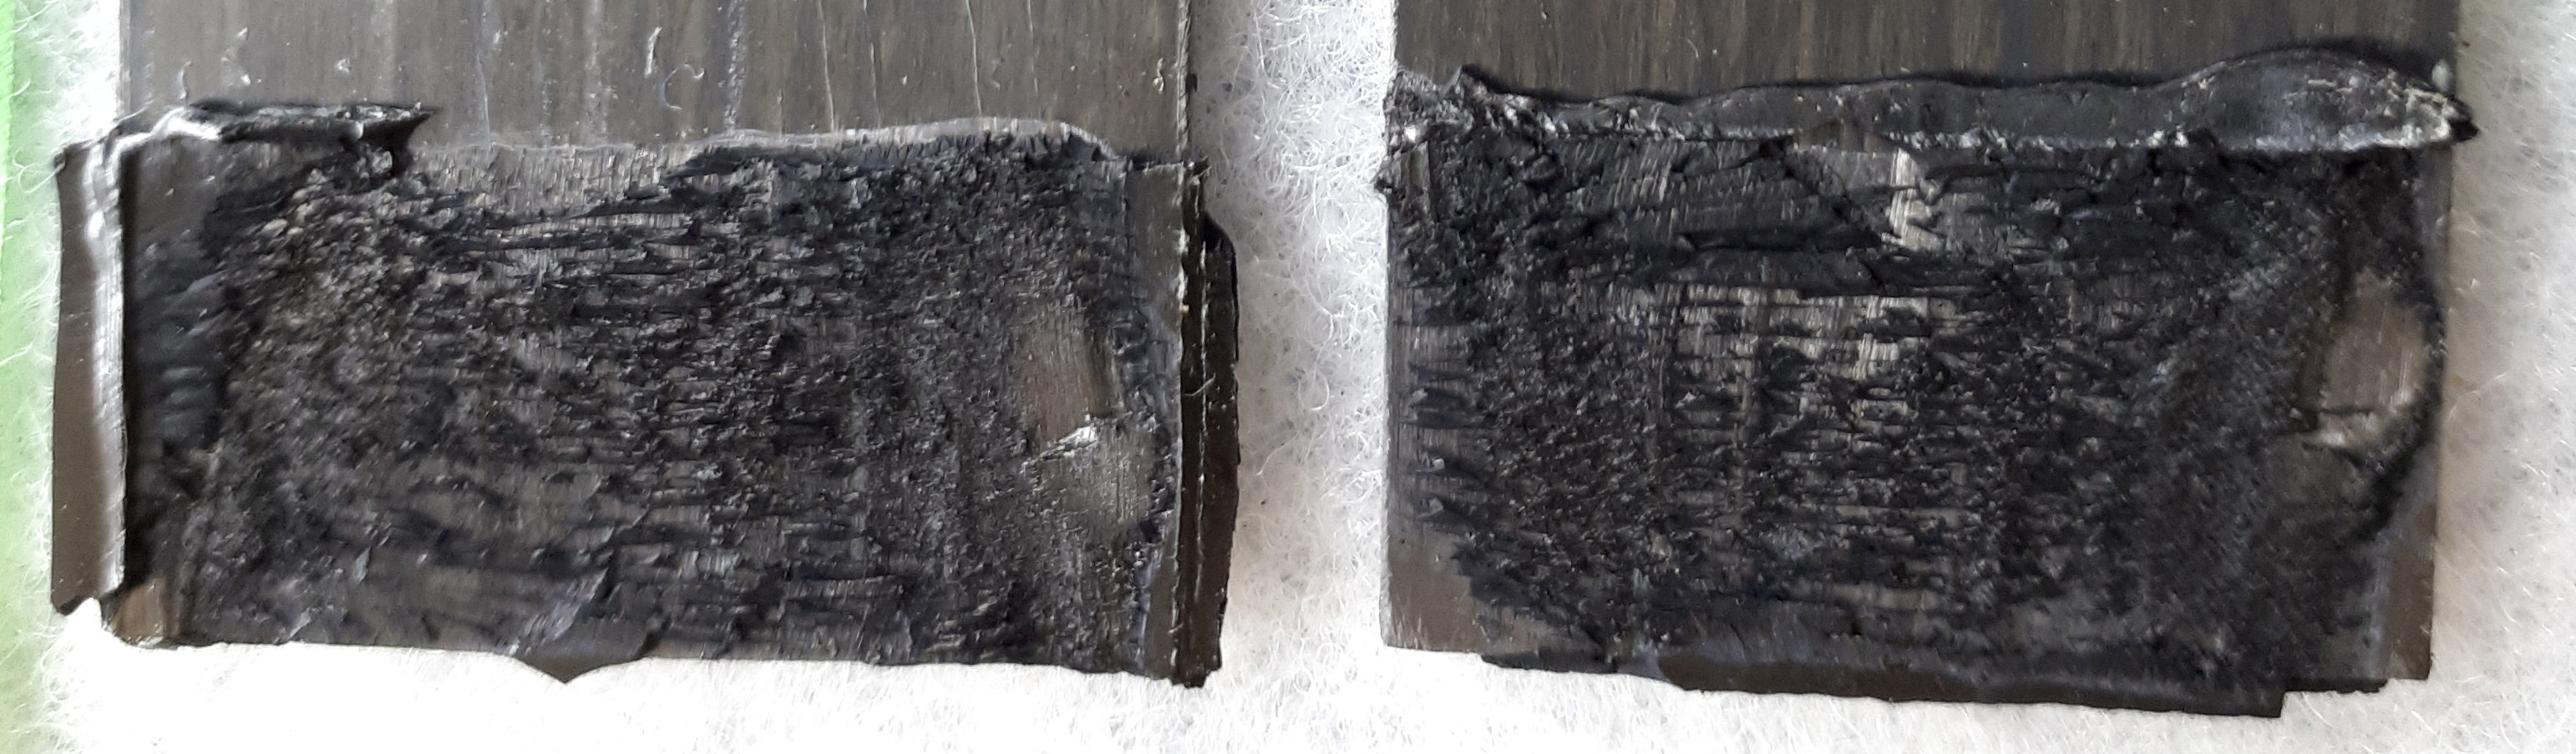
\includegraphics[width=125mm]{350kW-90-10-150-3UD_crop.jpg}
		\caption{Mostly cohesive failure in a sample welded for \SI{90}{\s}}
		\label{fig:fracture_surface_90s}
	\end{subfigure}%	
	\caption{Fracture surface of specimens welded at \SI{350}{\kW\per\square\metre} with \SI{1.5}{\mm} clamping distance \cite{Brassard2018_figshare_article1}}
	\label{fig:fracture_surface}
\end{figure}

\begin{figure}[h]
	\center
	\captionsetup{width=78mm}
	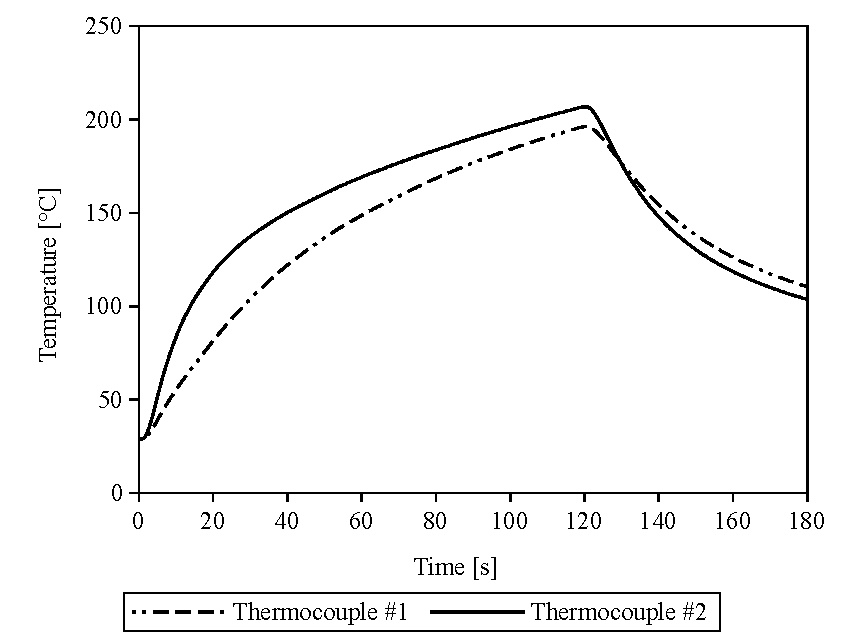
\includegraphics[width=3.25in]{temp_welding_350kw.pdf}
	\caption{Evolution of the temperature during the welding process at \SI{350}{\kilo\watt\per\square\metre} for \SI{120}{\second} \cite{Brassard2018_figshare_article1}}
	\label{fig:temp_350kW_120_10_150_3UD}
\end{figure}

\FloatBarrier
\clearpage
%%%%%%%%%%%%%%%%%%%%%%%%%%%%%%%%%%%%%%%%%%%%%%%%%%%%%%%%%%%%%%%%%
							\section*{Tables}
%%%%%%%%%%%%%%%%%%%%%%%%%%%%%%%%%%%%%%%%%%%%%%%%%%%%%%%%%%%%%%%%%
\FloatBarrier

\begin{table}[htb]
\centering
%\resizebox{88mm}{!}{
\begin{tabular}{@{}lrr@{}}
\toprule
Voltage 				& Electric							& Maximum  				\\ 
 						& field								& surface 				\\ 
 						& 										& temperature 			\\
{[}\si{\volt}{]} 	& {[}\si{\volt\per\metre}{]} 	& {[}\si{\celsius}{]}	\\ \midrule
10 						& 400									& 44 						\\
15						& 600									& 97 						\\
20 						& 800									& 155 						\\
25 						& 1000									& 223 						\\
30 						& 1200									& \textgreater 270 	\\ \bottomrule
\end{tabular}%}
\caption{Electrical results from the experimental validation}
\label{tab:results_lab}
\end{table}

\begin{table}[H]
\centering
\resizebox{\textwidth}{!}{
\begin{tabular}{@{}lllcccc@{}}
\toprule
Clamping distance	& Values			&						& \multicolumn{4}{c}{Time}																\\
{[}\si{\mm}{]}		&					&						& \multicolumn{4}{c}{{[}\si{\s}{]}}													\\
						&					&						& 60					& 70					& 90					& 120					\\ \midrule
0						& LSS				& {[}\si{\MPa}{]}	&						&						&						& \num{14.5(13)}	\\
						& Welded area	& {[}\%{]}			&						&						&						& \num{85(2)}		\\
1						& LSS				& {[}\si{\MPa}{]}	&						&						&						& \num{13.0(44)}	\\
						& Welded area	& {[}\%{]}			&						&						& 						& \num{83(7)}		\\
1.5						& LSS				& {[}\si{\MPa}{]}	& \num{16.4(78)}	& \num{18.6(20)}	& \num{15.5(38)}	& \num{19.6(35)}	\\
						& Welded area	& {[}\%{]}			& \num{57(20)}		& \num{74(10)}		& \num{87(1)}		& \num{78(2)}		\\ \bottomrule
\end{tabular}}
\caption{LSS and fractography analysis reported as average values $\pm$ standard deviation \cite{Brassard2018_figshare_article1}}
\label{tab:SLS_and_fractography_results}
\end{table}


\FloatBarrier
\clearpage


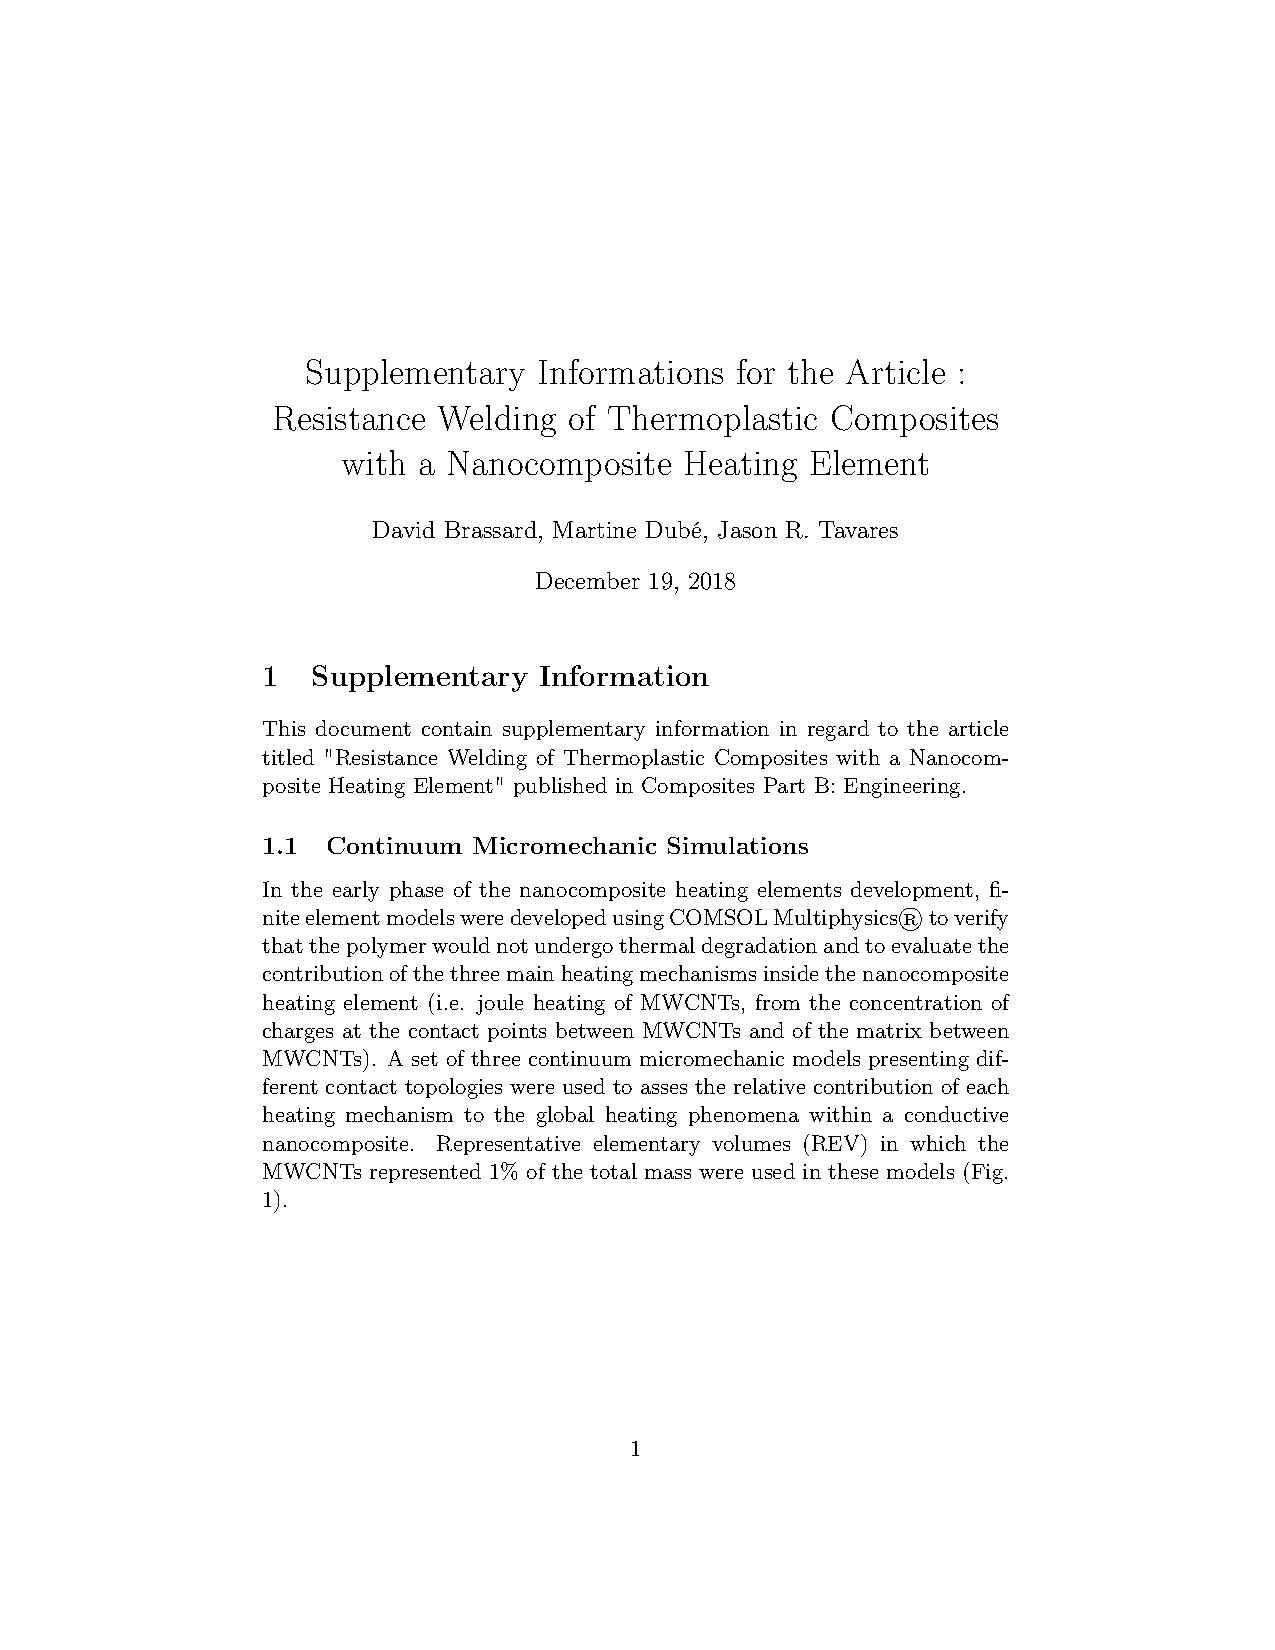
\includepdf[pages=-]{Supplementary_Information.pdf}

\end{document}
